\FloatBarrier
\subsection{Question 3}
In this section, we place the desired poles as demonstrated in \autoref{code:pp31}. The step response of the resulting closed-loop system is shown in \autoref{fig:pp31}. Using the pulse input generated in the previous section, the system output and control signals are plotted in \autoref{fig:pp32}. As shown, the desired pole locations effectively cancel the zeros of the original discrete system.

\begin{code}
	\begin{matlabcode}{firstnumber = 22}
	desired_poles = [roots(Gz.num{1}); 0.8];  % Cancel zeros with poles and add fast pole
	
	% Compute state feedback gain
	K = place(A, B, desired_poles);
	
	% Create closed-loop system with precompensator
	sys_ol = ss(A, B, C, D,sampleTimeIntervals);
	sys_cl = ss(A-B*K, B, C, D,sampleTimeIntervals);
	sys_cl = minreal(sys_cl);
	% Adjust DC gain for unity steady-state
	kr = 1/dcgain(sys_cl);
	sys_cl = ss(A-B*K, B*kr, C, D,sampleTimeIntervals);
	\end{matlabcode}
	\captionof{listing}{Pole placement with cancellation}
	\label{code:pp31}
\end{code}

\begin{figure}
	\centering
	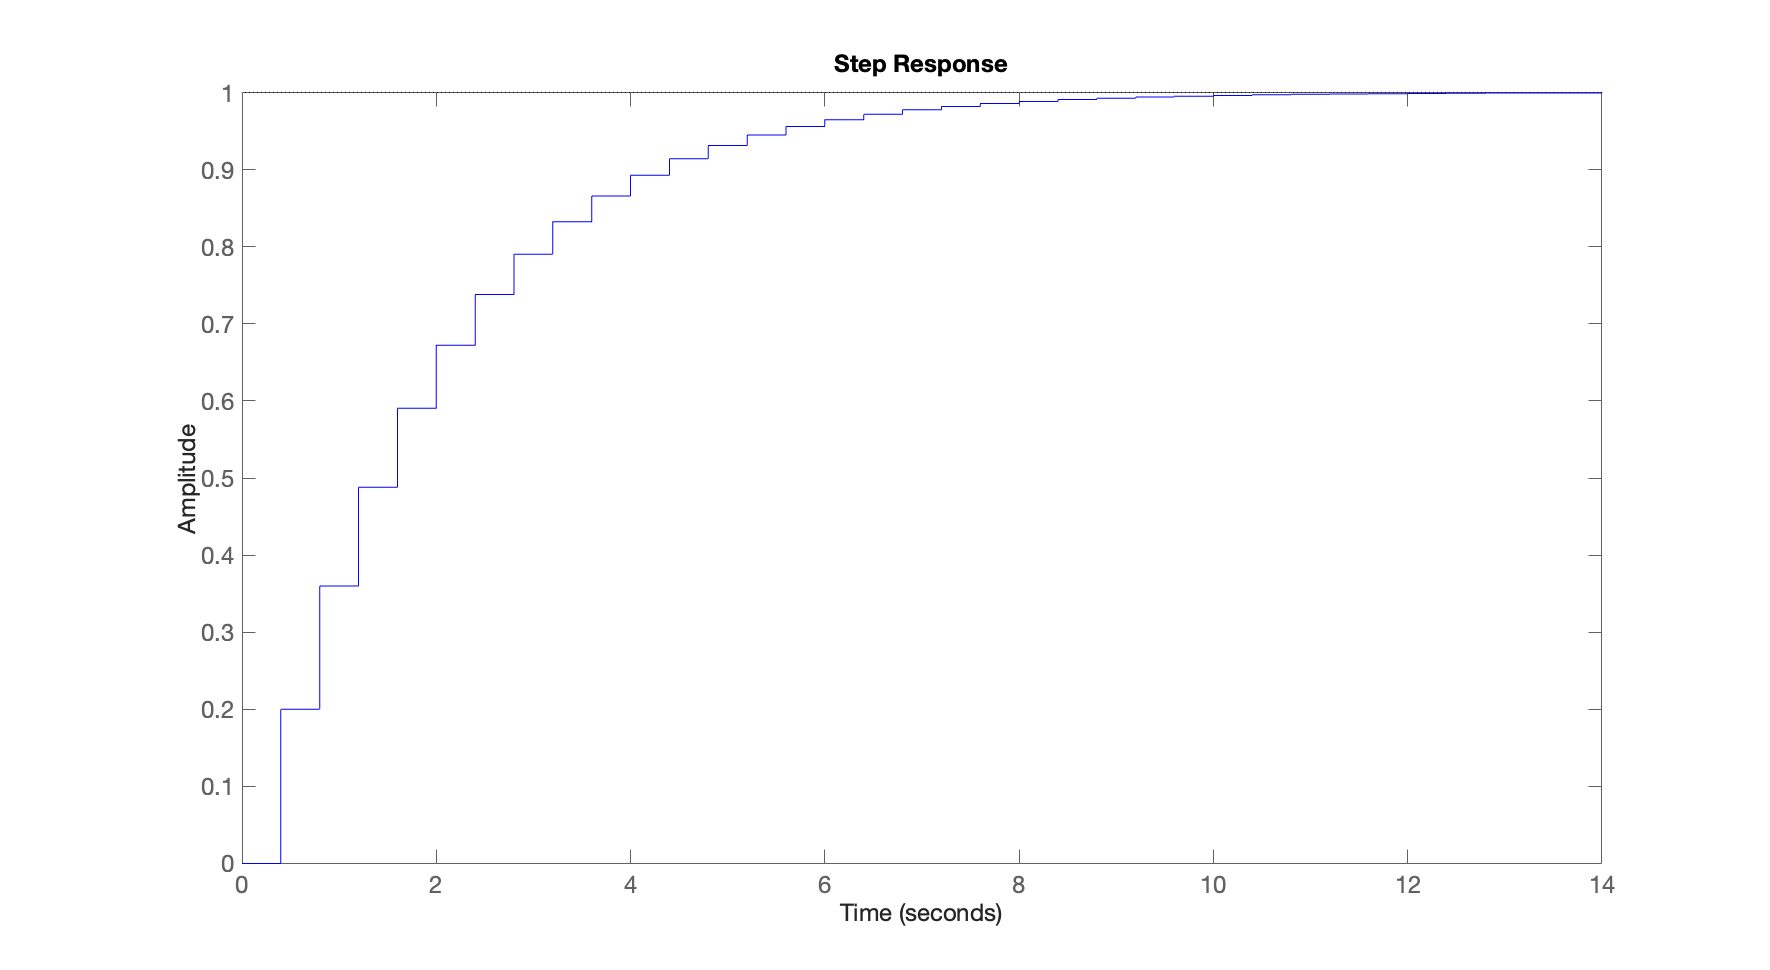
\includegraphics[width=\textwidth]{images/pp31.png}
	\caption{Step response of closed system with cancellation}
	\label{fig:pp31}
\end{figure}

\begin{figure}
	\centering
	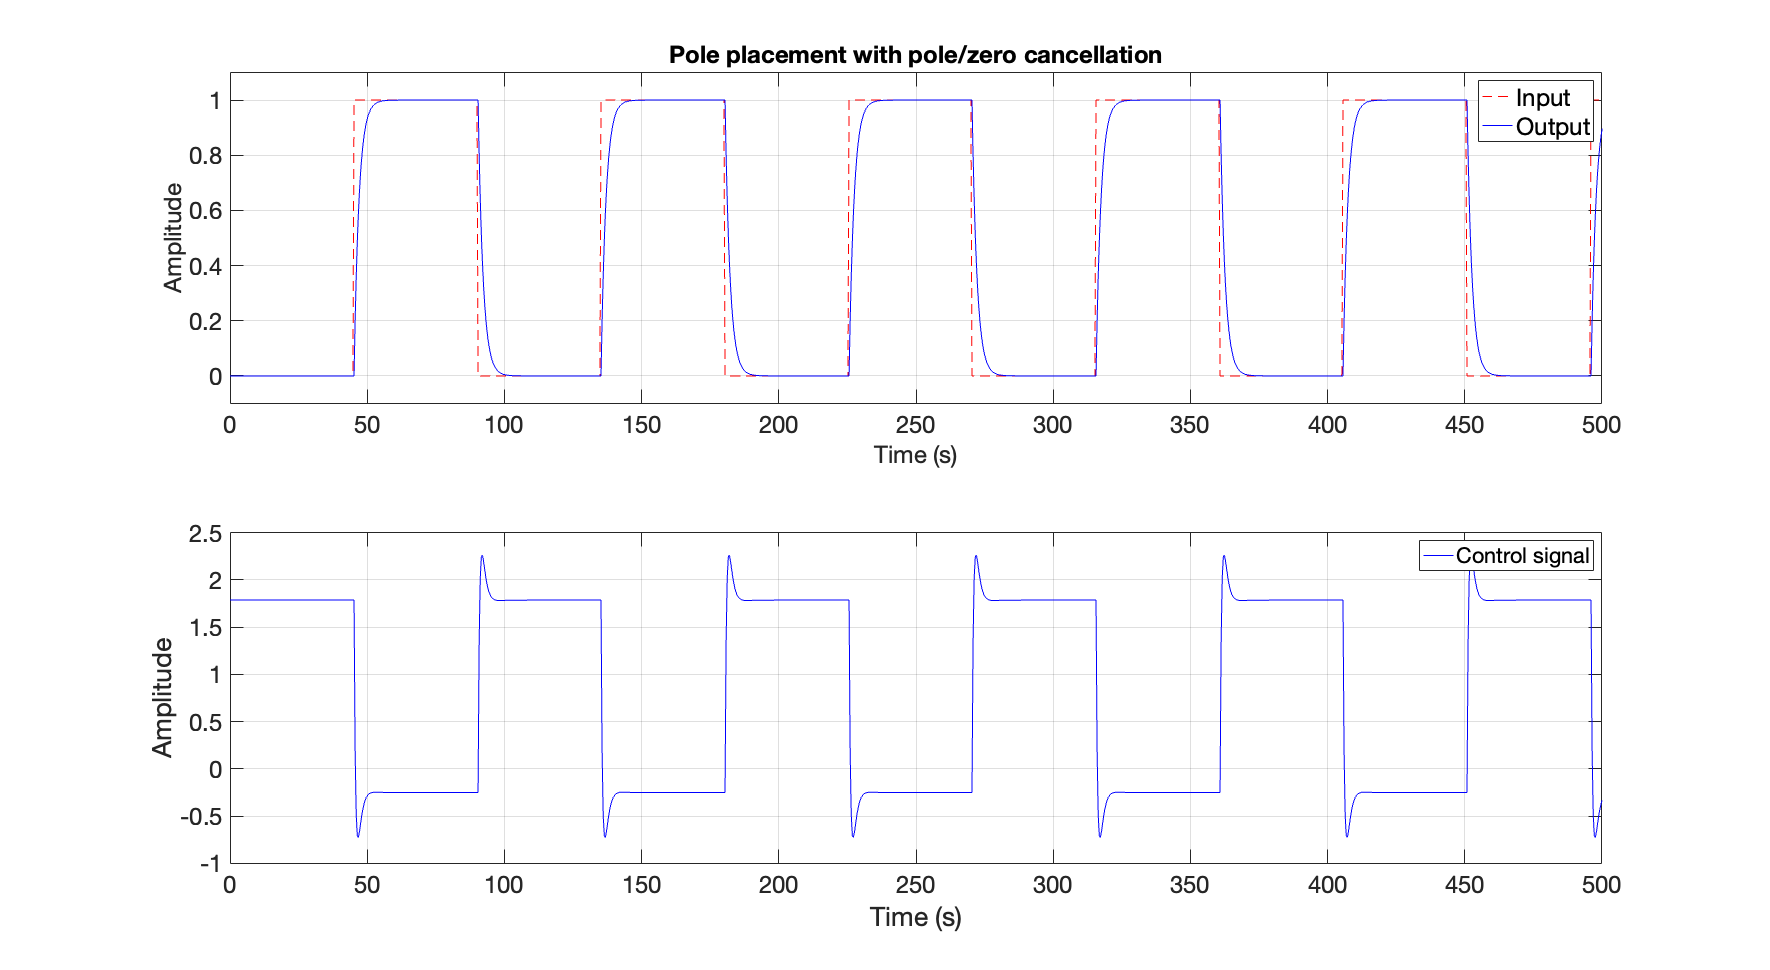
\includegraphics[width=\textwidth]{images/pp32.png}
	\caption{Pulse response of closed system with cancellation}
	\label{fig:pp32}
\end{figure}

\noindent The code for this section is available at \lstinline|assignment2/part1/PP1_3.m|. 
